\subsection{Authentication} \label{authentication_sota}
Authentication is the process of confirming and verifying someone's identity. In this section, we consider \acrlong{oidc} and FIDO as the two main technologies that can be used for online authentication. Afterwards, the NIST framework is presented, as it defines a useful classification model for authentication procedures, based on their security level.

\subsubsection{OpenID Connect}

%REFERENCE NAME TO OPENID STANDARD "Final: OpenID Connect Core 1.0 incorporating errata set 1"
\acrfull{oidc} is an authentication layer standard developed by OpenID Foundation. Current version is OpenID Connect 1.0, which has been proposed in November 2014~\cite{Sakimura2014Final:1}. \acrshort{oidc} is an extension and builds on top of the OAuth 2.0’s authorisation process, which is an authorisation standard and has been described in Section \ref{sec:OAuth_2}. 

As already mentioned, OAuth 2.0 is designated for authorisation but at the time it has been ‘misused’ for authentication purposes by tweaking it and developing different extensions~\cite{RicherUser2.0}. Therefore, there was a need for simple authentication standard which would build on top of the OAuth and that is \acrshort{oidc}.

The purpose of the \acrshort{oidc} is to allow the Client to authenticate (verify the identity) of the user, using the Authorisation server, which also provides identity information of the user, while OAuth 2.0 is being used to obtain access tokens and use them to access resources which are protected~\cite{OpenIDSpecs}. Technically speaking \textit{“OpenID Connect specifies a RESTful HTTP API, using JSON as a data format”}~\cite{OpenIDSpecs}.

Lets take an example of an user accessing a web service which requires log-in (also called \acrfull{rp}). The user needs to log-in first, e.g. using \acrfull{ms} account. User is redirected to the \acrfull{op}, where he has to enter his credentials and afterwards is requested to grand a permission for the service to access specific data from the \acrshort{ms} account, this happens on the Authorisation server
%(\acrshort{op} and Authorization server is the same entitity)
. If the authentication of the user is successful, \acrshort{op} provides \acrfull{rp} with \textit{id\_token} which verifies user’s identity and bears basic user’s information (e-mail, name, birthday, etc.). This \textit{id\_token} is in form of \acrfull{jwt} which defines a way of conveying data as \acrshort{json} object between parties securely, compactly and self-contained. Other token which is obtained during the process is \textit{Access Token}. User is then redirected to post login \acrshort{url}. If the  \acrshort{rp} needs to access protected resources, it uses the obtained \textit{Access Token} and the process continues using OAuth flow explained in Section \ref{sec:OAuth_2}.
\subsubsection{FIDO2}

Fast Identity Online Alliance (\acrshort{fido} Alliance) is an organization developing authentication standards. Protocols like \acrfull{u2f}, \acrfull{uaf} or \acrshort{fido}2 are products of \acrshort{fido} Alliance and its partners. The main aim of \acrshort{fido} is to create phishing-proof, password-less and secure standards. \acrshort{u2f} and \acrshort{uaf} has been proposed in 2014(REF), both being updated and having new versions over time however, the focus will be put towards the newest \acrshort{fido}2 project and its specification rather than older standards.

% TODO add figure reference
The \acrshort{fido}2 project’s aim is to provide phishing-proof, password-less, secure and simple authentication protocol. Fundamental components of \acrshort{fido}2 are WebAuthn which is the \acrshort{api} for a client (by \acrshort{w3c}) and \acrshort{ctap} (by \acrshort{fido}), the \acrshort{api} for the authenticator. These define an abstraction layer which allows strongly authenticated credentials. Therefore, any supported client, being it a native application or browser, running on client’s device and any supported authenticator, being it a build in or roaming authenticator connected to the device via \acrshort{nfc}, \acrshort{ble} or \acrshort{usb}, can use a standardized method to authenticate the user. There are several entities involved in the process of registering and subsequently authenticating the user as it can be seen in Figure XY.

% TODO add reference
\begin{figure}[ht]
    \centering
    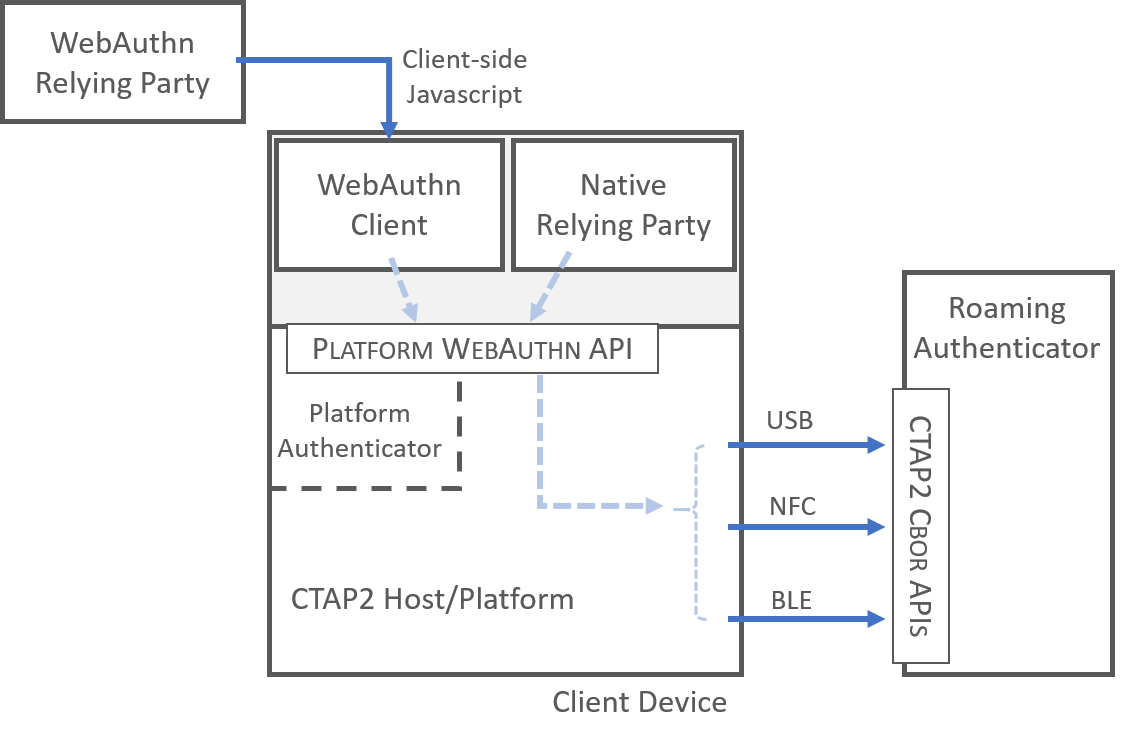
\includegraphics[width=.95\textwidth]{00images/FIDO2_Overview.png}
    \caption{Explanation. From~\cite{}SOURCE}
    \label{fig:fido2_overview}
\end{figure}

\paragraph{Client Device} 
is a hardware which is hosting the authentication via built in or roaming authenticator and communicates with a relying party. Example of such devices are laptops or smartphones. 

\paragraph{Roaming Authenticator} 
is an authenticator which can be connected to different client devices using \acrshort{ble}, \acrshort{nfc} or \acrshort{usb} interfaces. To communicate with a client device, \acrshort{ctap}1 or \acrshort{ctap}2 can be used.

\paragraph{Platform Authenticator} 
is built in on a client device and can only be used with a given device. Example of such authenticators are fingerprint scanners or facial recognition.

\paragraph{Relaying Party} 
is an application or service which requests authenticated credentials. It can be a native or web application.

\paragraph{\acrshort{ctap}2}
\acrlong{ctap} 2 (\acrshort{ctap}2) is the newest version of the \acrshort{ctap} protocol, which is backward compatible the preceding \acrshort{ctap}1/\acrshort{u2f} protocol by mapping \acrshort{ctap}2 request to \acrshort{ctap}1/\acrshort{u2f} and vice versa for responses, unless the relaying party requests a parameter which is \acrshort{ctap}2 specific. 

The \acrshort{ctap}2 specifies the application layer protocol so that authenticator and client device can communicate, as well as it defines how transport layer connection with different physical authenticators should be set up in accordance with the application layer protocol. This enables external devices to be used as authenticators and work with WebAuthn with applications and services.

% TODO add reference
The biggest improvements of \acrshort{ctap}2 over \acrshort{ctap} is the option to verify the user using biometrics or PIN. On top of that, besides storing a private key, devices are capable of storage of associated metadata which allows login even without typing an username. Android phones with android 7.0 and higher can be used as authenticators with their fingerprint or biometric scanners, thanks to a support of Trusted Platform Modules.(REF)

\paragraph{WebAuth} 
Web Authentication (WebAuthn) is the new web standard published on 4th March 2019  by \acrshort{w3c} which defines web \acrshort{api} which enables web browsers and platforms to enable external authenticators using \acrshort{fido} authentication. It standardizes the public-key authentication between users and web applications or services, so it is being used for communication between the client device and a RP.

When a user wants to use authentication with \acrshort{fido}2, given application or website must support it in the first place. User can create a new account or use an already existing one and associate it with the \acrshort{fido}2 authenticator. The authenticator, whether it is a roaming or built-in one, creates cryptographic key pair (private and public key) on user request which has to be confirmed by a user gesture, e.g. fingerprint, biometrics, PIN, touch. Key pair is then created, and the private key is securely stored on the authenticator while the public one, along with associated account details is sent to a server for storage.

% TODO change figure reference
In figure XYZ below, the high level sequence diagram of \acrshort{fido}2 authentication is shown. When a user wants to log-in to a service the relying party sends Credential ID and a challenge to a client, which then forwards this data to authenticator along with Relying party ID and Token binding. In order to proceed with authentication, user's gesture is required. Relying party ID counters the man-in-the-middle attack, making sure that it is always the same party the authentication is done with. Having Credential ID allows to have multiple accounts associated with the same key for the same service and have different key pair for each of the accounts. Authenticator then looks up the private key based on the Credential ID and Relying party ID, which is then used to sign the payload. The signed payload and a signature counter are sent then as an assertion to the client, which forwards it to the relying party together with the initial request. The relying party then verifies the signature with the public key of given account and logs in the user. The signature counter secures the authentication from authenticator clones. In case that the authenticator is cloned and an identical authenticator is produced by a malicious party, incrementing the counter at each sign-in ensures that the state of the original authenticator and its clone divert at some point. Therefore, if the clones is used at some point, it has lower counter than the is supposed to and gets detected and user gets notified.

% TODO add figure source
\begin{figure}[ht]
    \centering
    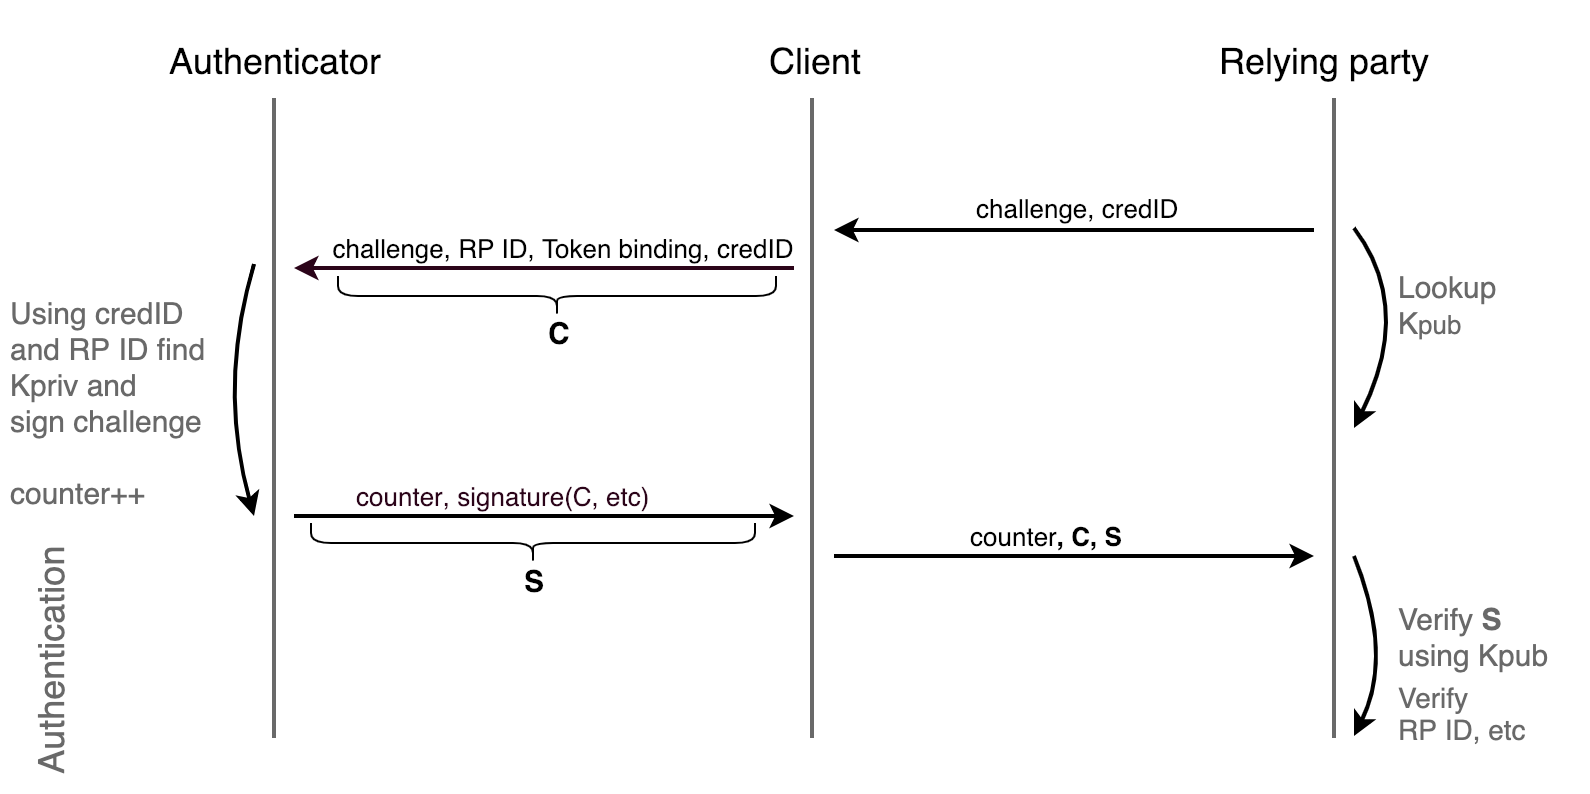
\includegraphics[width=.95\textwidth]{00images/FIDO2_Authentication.png}
    \caption{Explanation. From~\cite{}SOURCE}
    \label{fig:fido2_authentication}
\end{figure}
\subsubsection{NIST Digital Identity Guidelines}

The \acrfull{nist} developed a set of guidelines, intended primarily to govern how public authorities in the US implement digital authentication in non-national-security scenarios. However, it was adopted by a wider community, spanning out of the government sector~\cite{Grassi2017GovernmentCollaboration}.

The guidelines contain three volumes, covering three distinct areas of authentication:
\begin{enumerate*}[label=(\roman*)]
    \item SP 800-63A focused on Enrolment and Identity Proofing;
    \item SP 800-63B centred around Authentication and Lifecycle Management; and
    \item SP 800-63C covering Federation and Assertions.
\end{enumerate*}
The guidelines advertise the use of authentication to mitigate risks of unauthorised access to protected resources, but also promote minimising the collection of \acrfull{pii} and use of pseudonymous information whenever possible~\cite{Grassi2017Digital3}.

The guidelines define a Digital Identity Model (Figure~\ref{fig:nist-model}), which is useful to distinguish the various types of roles and activities within an authentication system. On the left side of the model there is a \acrfull{csp}. \acrshort{csp} is an entity that issues electronic credentials and registers user's \textit{authenticator} (authenticator is something that the user has or controls). On the right side of the model is the verifier, whose task is to authenticate users by validating binding of their authenticators to their credentials~\cite{Grassi2017Digital3}.

 \begin{figure}[ht]
    \centering
    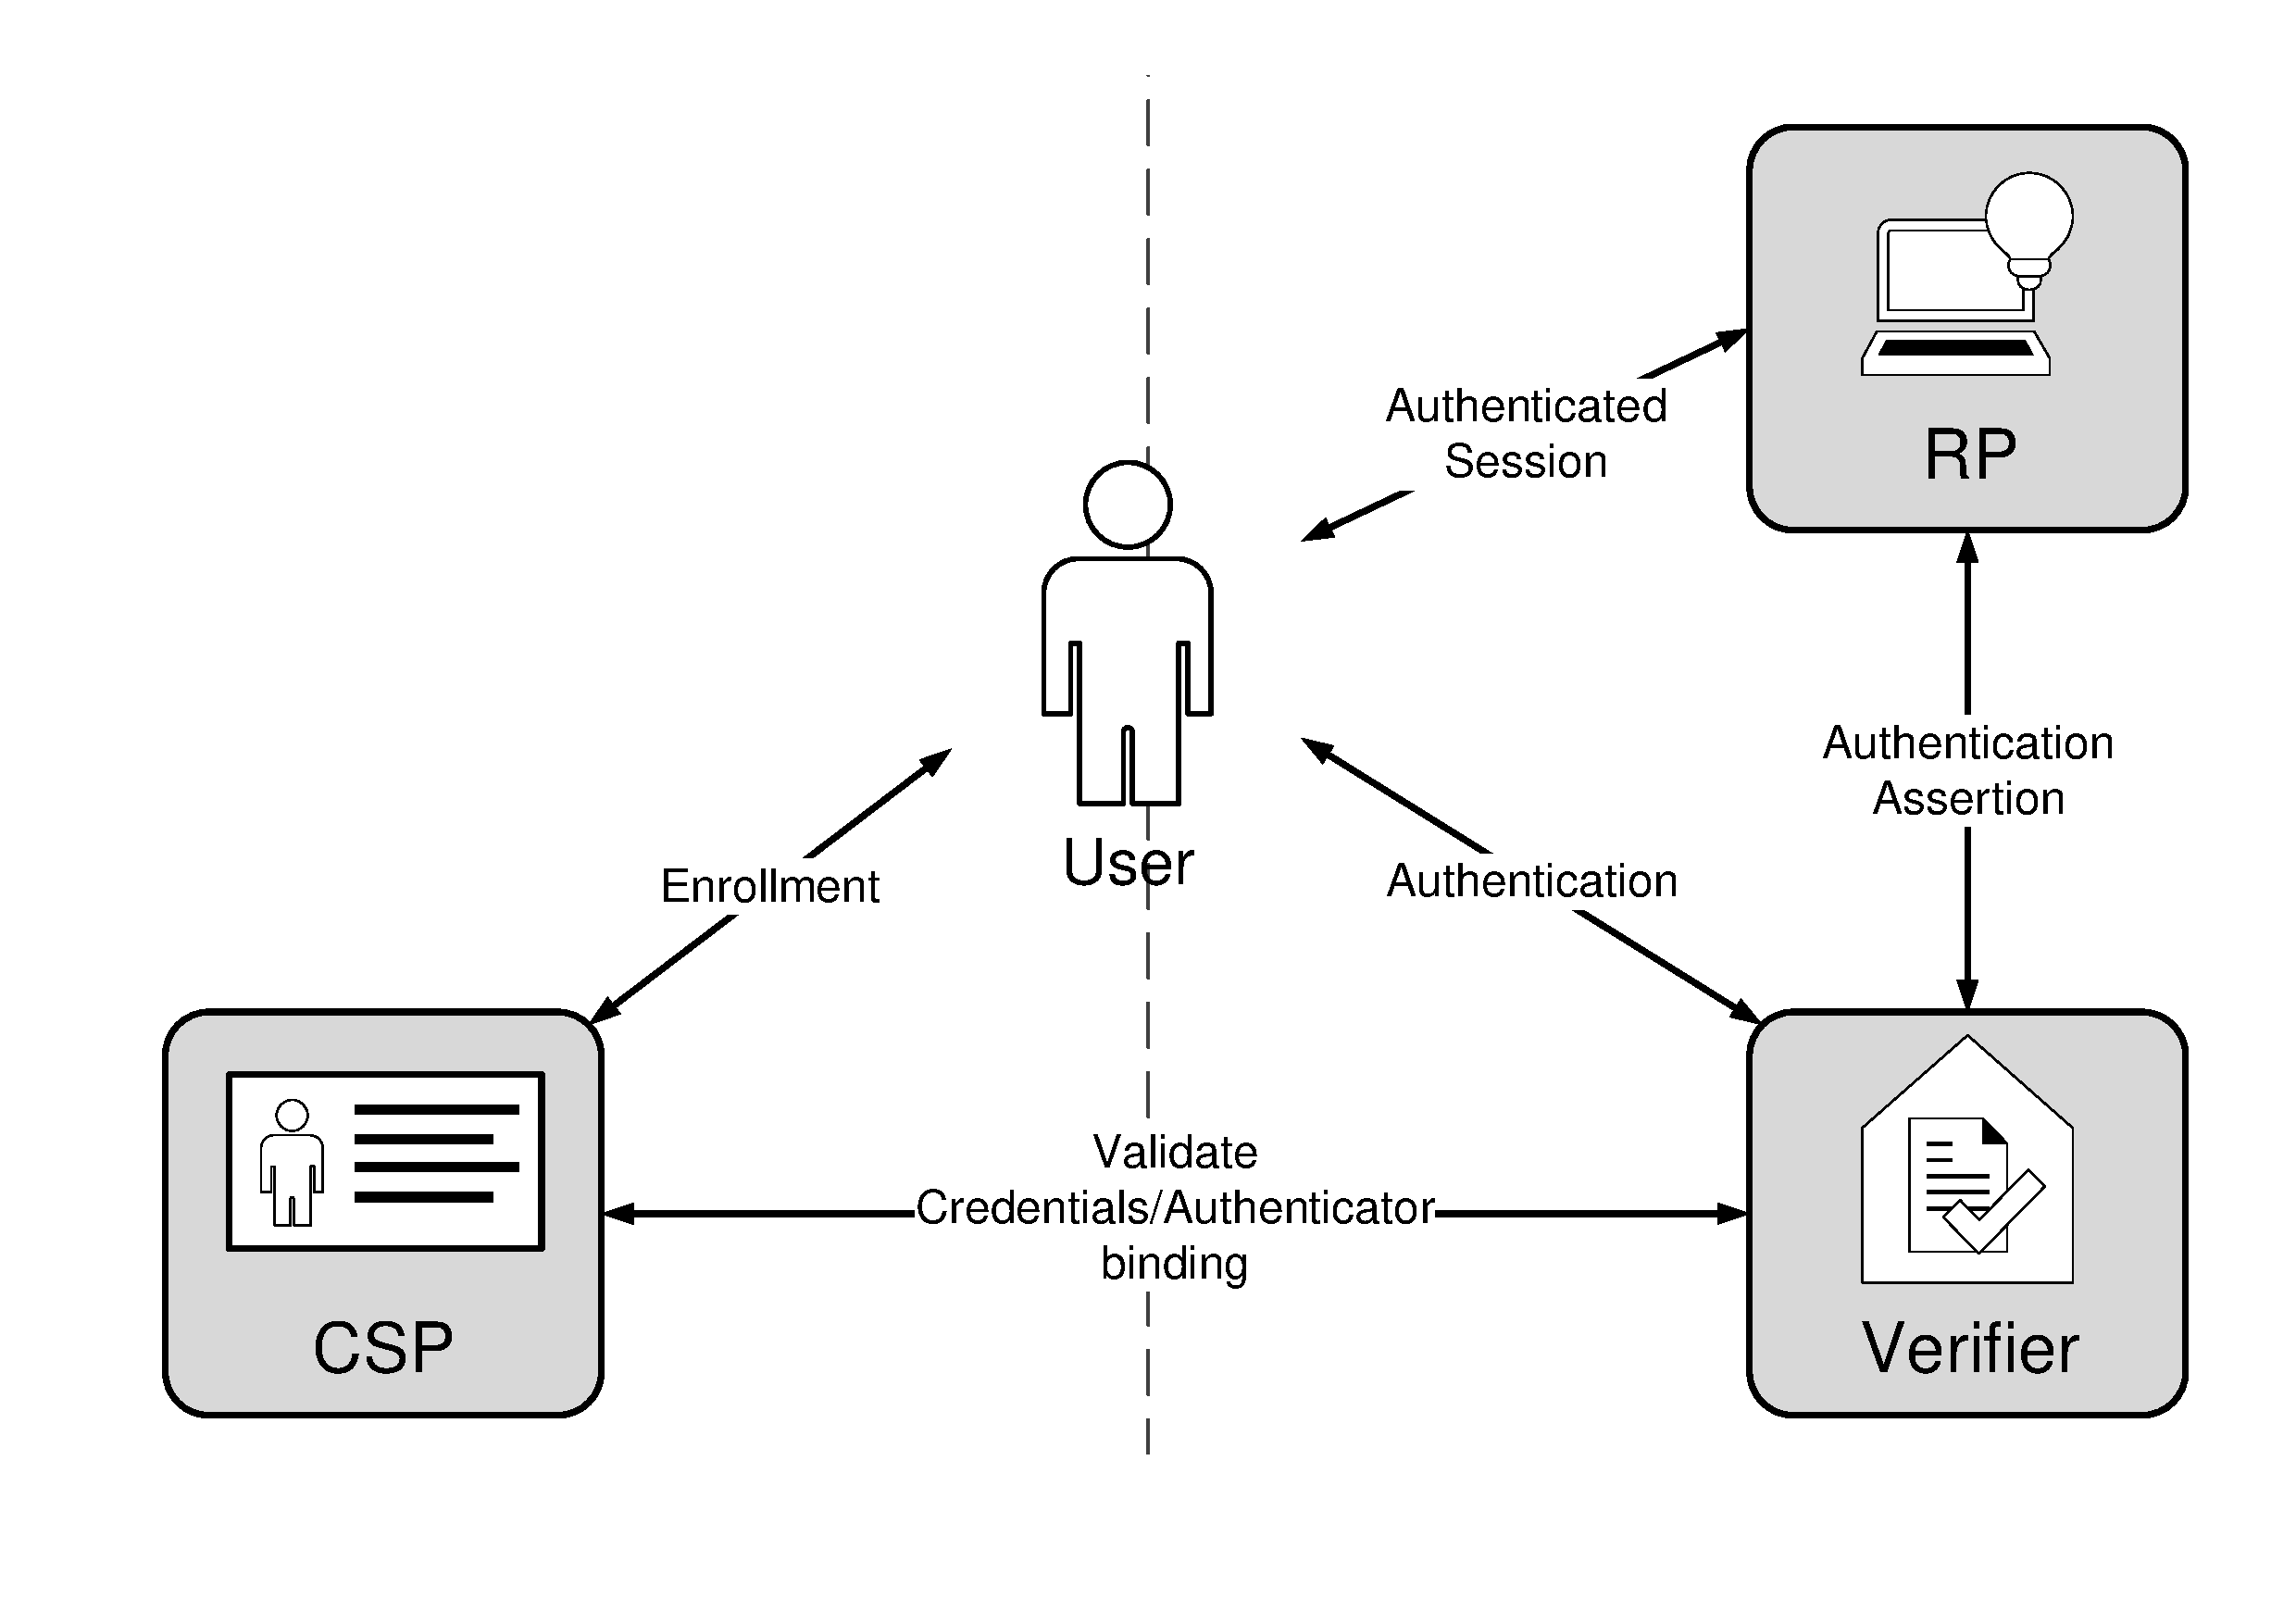
\includegraphics[width=.95\textwidth]{nist-simplified}
    \caption{Digital Identity Model (simplified). The left side of the figure represents enrolment of the user with the \acrshort{csp}. The right part of the user represents authentication with the verifier, before an authenticated session is established between the user and the \acrshort{rp}. Taken from~\cite{Grassi2017Digital3} (edited).}
    \label{fig:nist-model}
\end{figure}

\paragraph{SP 800-63A}
This volume of the Digital Identity Guidelines defines three Identity Assurance Levels (IALs) and requirements on identity proofing for each level. The \acrshort{ial}1 requires no verification of assertions provided by the user. \acrshort{ial}2 requires either remote or physically-present verification of assertions made by the user, while \acrshort{ial}3 requires manual verification by a trained person, representing the \acrshort{csp}~\cite{Grassi2017DigitalProofing}.

\paragraph{SP 800-63B}
The B volume of the Guidelines defines three Authenticator Assurance Levels (AALs).

To authenticate themselves in AAL1, the user needs to demonstrate control of one authenticator. This must be done through a secure authentication protocol.

In AAL2, the user must demonstrate control of two distinct authenticators. This can be in a form of a multi-factor authenticator, or single-factor possession-based authenticator together with a memorised password. Cryptographic techniques defined in~\cite{Evans2001SECURITYMODULES} must be used.

In AAL3, a hardware-based authenticator must be used in addition to requirements of AAL2. Furthermore, one of the authenticators used must be resistant to attacks attempting to impersonate the user.

\paragraph{SP 800-63C}
The C volume of the guidelines describes the use of assertions for identity federation across several \acrshort{rp}s~\cite{Grassi2017DigitalAssertions}. This enables the user to use services provided by several \acrshort{rp}s, while maintaining only a single identity at one \acrshort{idp}. The volume also describes three Federation Assurance Levels, however we do not cover these in this report.